% ============================================================
% 第16章：闭区间上连续函数的性质——四大定理
% ============================================================

\chapter{闭区间上连续函数的性质——四大定理}

\begin{applicationbox}
\textbf{学完本章你能做什么？}
\begin{enumerate}
  \item 掌握闭区间上连续函数的\textbf{四大定理}
  \item 理解\textbf{介值定理}——中间值一定有解
  \item 理解\textbf{最值定理}——闭区间上一定有最大值和最小值
\end{enumerate}
\end{applicationbox}


% ============================================================
\section{四大定理}
% ============================================================

\begin{theorembox}[1. 有界性定理]
若 \(f\) 在 \([a,b]\) 上连续，则 \(f\) 在 \([a,b]\) 上有界。

\textbf{ε-δ 证明：} 由 \(f\) 在 \([a,b]\) 上 ε-δ 连续（第15章），
取 \(\varepsilon=1\)，则对每个 \(x\in[a,b]\)，存在 \(\delta_x>0\) 使
\(|y-x|<\delta_x\) 时 \(|f(y)-f(x)|<1\)。
开区间族 \(\{U(x,\delta_x)\}_{x\in[a,b]}\)（即 \((x-\delta_x,x+\delta_x)\)）构成 \([a,b]\) 的开覆盖。
由海涅-博雷尔定理（第15章第5.3节），存在有限子覆盖 \(U(x_1,\delta_{x_1}),\ldots,U(x_n,\delta_{x_n})\)。
取 \(M=\max\{|f(x_1)|,\ldots,|f(x_n)|\}+1\)，则对任意 \(y\in[a,b]\)，
\(y\) 属于某个 \(U(x_i,\delta_{x_i})\)，故 \(|f(y)|\le|f(x_i)|+1\le M\)，即 \(f\) 有界。\(\blacksquare\)
\end{theorembox}

\begin{theorembox}[2. 最值定理（最大值最小值定理）]
若 \(f\) 在 \([a,b]\) 上连续，则 \(f\) 在 \([a,b]\) 上一定能取到最大值和最小值。

\textbf{ε-δ 证明：} 由有界性定理知 \(f\) 有上确界 \(M=\sup\{f(x):x\in[a,b]\}\)。
假设 \(f(x)<M\) 对所有 \(x\in[a,b]\) 成立，则 \(g(x)=\frac1{M-f(x)}\) 在 \([a,b]\) 上 ε-δ 连续（分母不为 0）。
但 \(g(x)\) 无界（因为 \(f(x)\) 可任意接近 \(M\)），与有界性定理矛盾。
故存在 \(c\) 使 \(f(c)=M\)，即最大值可达。最小值同理。\(\blacksquare\)
\end{theorembox}

\begin{theorembox}[3. 介值定理]
若 \(f\) 在 \([a,b]\) 上连续，且 \(f(a) \neq f(b)\)，
则对 \(f(a)\) 和 \(f(b)\) 之间的任意数 \(k\)，
存在 \(c \in (a,b)\) 使得 \(f(c) = k\)。

\textbf{ε-δ 证明：} 设 \(f(a)<k<f(b)\)。令集合 \(S=\{x\in[a,b]:f(x)<k\}\)，
则 \(S\) 非空（\(a\in S\)），有上界（\(b\) 为上界）。设 \(c=\sup S\)（上确界）。
由 \(f\) 的 ε-δ 连续性，若 \(f(c)<k\)，则存在 \(\delta>0\) 使
\((c,c+\delta)\) 内 \(f(x)<k\)，与 \(c\) 是上界矛盾；
若 \(f(c)>k\)，则存在 \(\delta>0\) 使 \((c-\delta,c+\delta)\) 内 \(f(x)>k\)，
与 \(c\) 是上确界矛盾。故 \(f(c)=k\)。\(\blacksquare\)
\end{theorembox}

\begin{theorembox}[4. 零点定理（介值定理的推论）]
若 \(f\) 在 \([a,b]\) 上连续，且 \(f(a) \cdot f(b) < 0\)（即一正一负），
则存在 \(c \in (a,b)\) 使得 \(f(c) = 0\)。
\end{theorembox}


% ============================================================
\section{介值定理的几何意义}
% ============================================================

\begin{examplebox}[1——介值定理]
\begin{center}
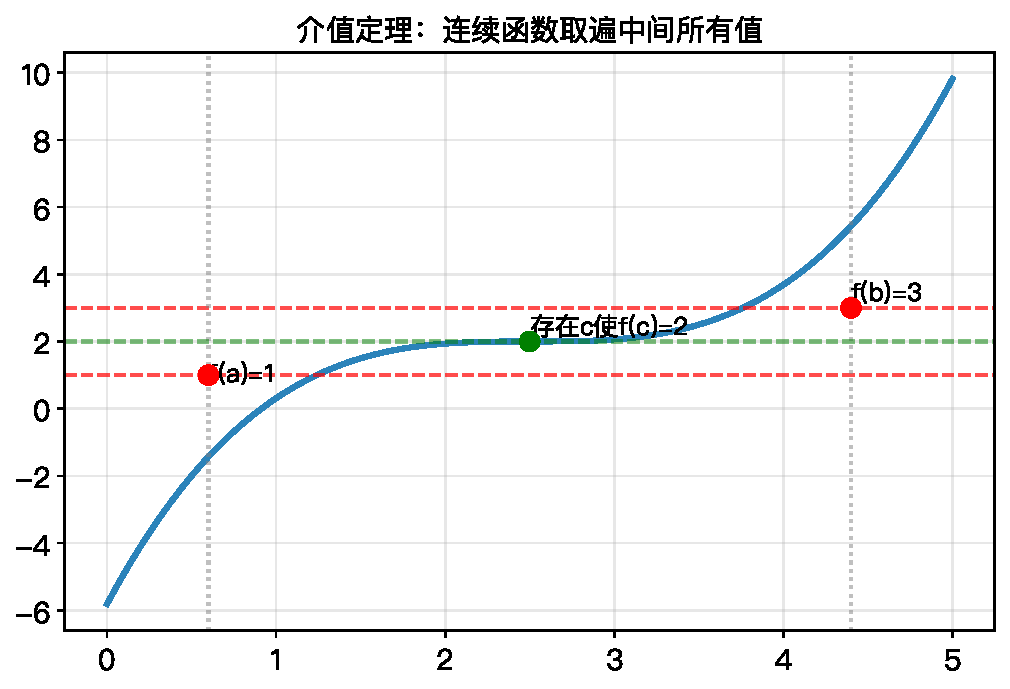
\includegraphics[width=0.7\textwidth]{figures/ch16_intermediate_value.pdf}
\end{center}

连续函数的图像从 \(f(a)=1\) 到 \(f(b)=3\)，中间不能断开，\
所以一定会经过 \(y=2\)。这就是介值定理——连续函数取遍中间所有值。
\end{examplebox}

\begin{examplebox}[2——零点定理的应用]
证明方程 \(x^3 - x - 1 = 0\) 在 \((1,2)\) 内有根。

\textbf{证明：} 令 \(f(x) = x^3 - x - 1\)。\\
\(f(1) = 1 - 1 - 1 = -1 < 0\)\\
\(f(2) = 8 - 2 - 1 = 5 > 0\)

\(f\) 在 \([1,2]\) 上连续，且 \(f(1)f(2) < 0\)。\\
由零点定理，存在 \(c \in (1,2)\) 使得 \(f(c) = 0\)，即 \(c\) 是方程的根。
\end{examplebox}


% ============================================================
\section{本章小结}
% ============================================================

\begin{progressbox}
\textbf{闭区间上连续函数的四大定理：}
\begin{itemize}
  \item 有界性定理：连续必有界
  \item 最值定理：连续必取最值
  \item 介值定理：连续必取中间值
  \item 零点定理：正负之间必有零点
\end{itemize}

这些定理直观上都是"一笔画"的直接推论。
\end{progressbox}

% ============================================================
% 习题
% ============================================================
\section{习题}

\begin{exercise}[0]
介值定理的条件是什么？
\end{exercise}
\begin{exercise}[0]
零点定理中，\(f(a)\) 和 \(f(b)\) 必须满足什么条件？
\end{exercise}
\begin{exercise}[0]
连续函数在闭区间上一定有最大值吗？
\end{exercise}
\begin{exercise}[0]
用零点定理判断：方程 \(x-1=0\) 在 \((0,2)\) 内有根吗？
\end{exercise}

\begin{exercise}[1]
证明方程 \(x^3 - 3x + 1 = 0\) 在 \((0,1)\) 内有根。
\end{exercise}
\begin{exercise}[1]
证明方程 \(\cos x = x\) 在 \((0,\pi/2)\) 内有根。
\end{exercise}
\begin{exercise}[1]
证明方程 \(e^x = 2 - x\) 在 \((0,1)\) 内有根。
\end{exercise}
\begin{exercise}[1]
判断：闭区间上的连续函数一定有界吗？
\end{exercise}

\begin{exercise}[2]
证明方程 \(x^5 - 3x + 1 = 0\) 在 \((0,1)\) 内有根。
\end{exercise}
\begin{exercise}[2]
证明方程 \(\ln x = x - 2\) 在 \((2,3)\) 内有根。
\end{exercise}
\begin{exercise}[2]
设 \(f\) 在 \([0,1]\) 上连续，\(f(0)=f(1)\)，证明存在 \(c\in(0,1)\) 使 \(f(c)=f(c+1/2)\)。
\end{exercise}
\begin{exercise}[2]
证明：奇次多项式至少有一个实根。
\end{exercise}

\begin{exercise}[3]
证明方程 \(x^3 + x - 3 = 0\) 在 \((1,2)\) 内有唯一实根。
\end{exercise}
\begin{exercise}[3]
设 \(f\) 在 \([0,1]\) 上连续且 \(0\le f(x)\le 1\)，证明存在 \(c\in[0,1]\) 使 \(f(c)=c\)（不动点定理）。
\end{exercise}
\begin{exercise}[3]
证明：若 \(f\) 在 \([a,b]\) 上连续且严格递增，则 \(f\) 的值域是 \([f(a),f(b)]\)。
\end{exercise}
\begin{exercise}[3]
设 \(f\) 在 \([0,1]\) 上连续，\(f(0)=1\)，\(f(1)=0\)，证明存在 \(c\) 使 \(f(c)=c\)。
\end{exercise}
\begin{exercise}[3]
方程 \(2^x = 4x\) 在 \((0,1)\) 和 \((3,4)\) 内是否有根？
\end{exercise}

\begin{exercise}[4]
证明：若 \(f\) 在 \([a,b]\) 上连续且 \(f([a,b])\subset[a,b]\)，则存在 \(c\) 使 \(f(c)=c\)。
\end{exercise}
\begin{exercise}[4]
设 \(f\) 在 \([0,2]\) 上连续，\(f(0)=f(2)\)，证明存在 \(c\in[0,1]\) 使 \(f(c)=f(c+1)\)。
\end{exercise}
\begin{exercise}[4]
证明：\(f(x)=x^n + x - 1\)（\(n\) 为正奇数）在 \((0,1)\) 内有根。
\end{exercise}
\begin{exercise}[4]
设 \(f\) 在 \([0,1]\) 上连续，证明 \(f\) 在 \([0,1]\) 上有最大值和最小值。
\end{exercise}
\begin{exercise}[4]
证明方程 \(\sin x = x-1\) 在 \((0,\pi)\) 内有根。
\end{exercise}

\begin{exercise}[5]
设 \(f\) 在 \([a,b]\) 上连续，\(x_1,x_2,\ldots,x_n\in[a,b]\)，
证明存在 \(c\in[a,b]\) 使 \(f(c)=\frac{f(x_1)+\cdots+f(x_n)}{n}\)。
\end{exercise}
\begin{exercise}[5]
证明：若 \(f\) 在 \(\mathbb{R}\) 上连续且 \(\lim_{x\to\pm\infty}f(x)=0\)，则 \(f\) 有最大值或最小值。
\end{exercise}
\begin{exercise}[5]
方程 \(x = \cos x\) 在 \((0,\pi/2)\) 内有几个根？
\end{exercise}
\begin{exercise}[5]
设 \(f\) 在 \([0,1]\) 上连续且 \(f(0)>1\)，\(f(1)<1\)，证明存在 \(c\) 使 \(f(c)=c\)。
\end{exercise}

\begin{exercise}[6]
证明：若 \(f\) 在 \([a,b]\) 上连续且单射，则 \(f\) 在 \([a,b]\) 上严格单调。
\end{exercise}
\begin{exercise}[6]
设 \(f\) 在 \([0,1]\) 上连续，\(f(0)=f(1)\)，证明对任意正整数 \(n\)，
存在 \(c\in[0,1]\) 使 \(f(c)=f(c+1/n)\)。
\end{exercise}
\begin{exercise}[6]
证明：若 \(f\) 在 \(\mathbb{R}\) 上连续且 \(\lim_{x\to\infty}f(x)=\infty\)，\(\lim_{x\to-\infty}f(x)=-\infty\)，
则对任意 \(y\in\mathbb{R}\)，存在 \(x\) 使 \(f(x)=y\)。
\end{exercise}

\begin{exercise}[7]
设 \(f\) 在 \([a,b]\) 上连续，\(g\) 在 \([a,b]\) 上连续且 \(g(a)<0<g(b)\)。
证明存在 \(c\in(a,b)\) 使 \(f(c)=f(c)g(c)\)。
\end{exercise}

